This section will tell you everything you need to know to start using the
embedded filesystems library on a TMS Digital Signal Processor from Texas Instruments.
The only thing that is required is that you have a McBSP port available, and that your DSP
support CLOCKSTOP mode, which is required to connect a SPI compatible device.

There are special DSP's from TI which have a special MMC/SD card controller, if you want to
use this special interface you will have to create a hardware endpoint for it. This section only
describes connecting an SD card to a normal McBSP port, since every TI DSP has at least one of them.

\subsubsection{Hardware}
Connecting the SD card to the McBSP is straightforward, you will have to make 4 data related
connections, Vcc and ground, resulting in a 6 wire interface.\\
\begin{tabular}{|l|l|l|l|l|}
	\hline
	\multicolumn{3}{|c|}{SD Card Interface}&\multicolumn{2}{|c|}{McBSP Interface}\\
	\hline
	1 & CS & Chip select & FSX & Frame Sync Transmit \\
	2 & MOSI & Master out Slave In & DX & Data transmit \\
	3 & GND & Supply Ground &&\\
	4 & Vcc & Supply voltage (3.3 Volt) &&\\
	5 & Clk & Clock & CLKX & Clock Transmit\\
	6 & GND & Supply ground &&\\
	7 & MISO & Master in Slave out & DR & Data receive \\
	8 & NC & Not connected &&\\
	9 & NC & Not connected &&\\
	\hline
\end{tabular}\\
You can optionally pull the DataIn and DataOut lines up to Vcc with a $10k\Omega$ resistor, but
we found that this was not required for operation.\\
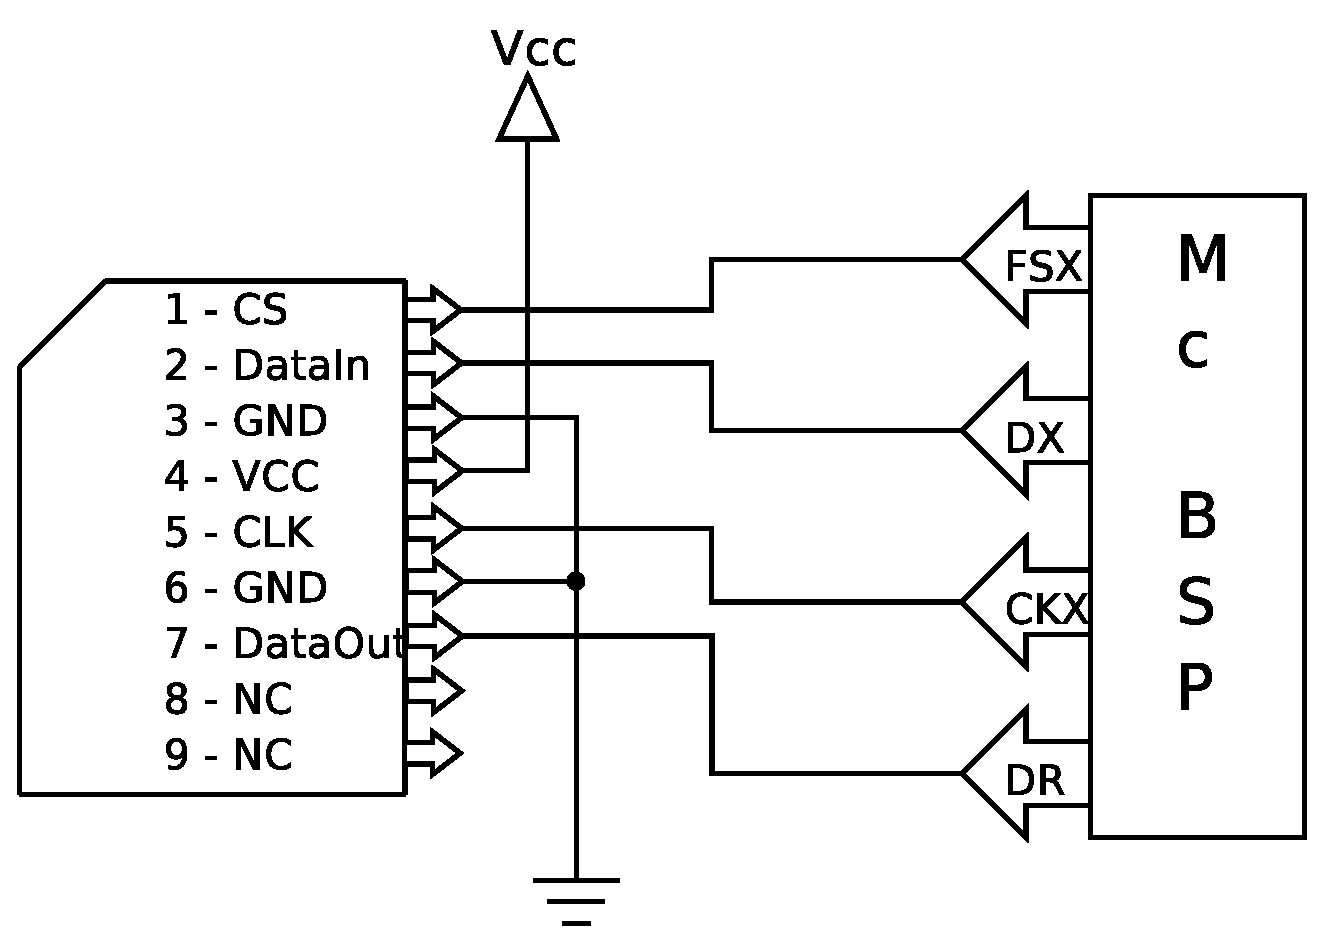
\includegraphics[scale=0.4]{schematics/sdcard.eps}\\
The frame sync from the McBSP port is used to select the card whenever a databyte has to be transferred, it is connected to the chip select of the SD card. The DX and DR pins are connected to the SDcard's DataIn and DataOut lines respectively. Finally the McBSP will have to generate a clock for
the SDcard so that it can perform operations, this is accomplished by connecting the clock transmit
line of the McBSP port to the CLK pin of the SDCard.

\subsubsection{McBSP configuration}
\begin{longtable}{|p{0.13\textwidth}|p{0.1\textwidth}|p{0.06\textwidth}|p{0.75\textwidth}|}
	
	\hline
	\multicolumn{4}{|c|}{
		\textbf{McBSP Register Explanations}
	} \\
	\hline
	\hline
	\endfirsthead
	
	\hline
	\multicolumn{4}{|c|}{\textbf{mcbsp registers (continued)}} \\
	\hline
	\endhead
	\hline
	\endfoot
	
	\hline 
	\endlastfoot

 	\multicolumn{3}{|c|}{SPCR}&
 	\multicolumn{1}{c|}{Serial Port Control Register}\\
 	\hline
 	Name & Bit & Value &\multicolumn{1}{c|}{Value \code{(0x00001800 | 0x00410001)}}\\
 	\hline
	RRST&\code{0}&\code{1b} & The serial port receiver is enabled \\
	XRST&\code{16}&\code{1b} & The serial port transmitter is enabled \\
	CLKSTP&\code{12:11}&\code{11b} & Clock starts on falling edge without delay(see CLKXM) \\
	GRST&\code{22}&\code{1b} & Sample rate generator is pulled out of reset \\
	\hline

 	\multicolumn{3}{|c|}{PCR}&
 	\multicolumn{1}{c|}{Pin Control Register}\\
 	\hline
 	Name &Bit & Value &\multicolumn{1}{c|}{Value \code{0x00000A0C}}\\
 	\hline
	CLKXP&\code{1} &\code{0b} & Transmit data on the rising edge ofthe clock\\
	FSXP&\code{3} &\code{1b} & Frame Sync (Chip select on SD card) is active low\\
	CLKXM&\code{9} &\code{1b} & McBSP is a master in SPI mode and generates the clock based on
	                            the sample rate generator\\
	FSXM&\code{10} &\code{1b} & Frame sync is determined by tge sample rate generator\\
	\hline

 	\multicolumn{3}{|c|}{RCR/XCR}&
 	\multicolumn{1}{c|}{Receive/Transmit Control Register}\\
 	\hline
 	Name &Bit & Value &\multicolumn{1}{c|}{Value \code{0x00010000}}\\
 	\hline
	RWDLEN&\code{7:5} &\code{000b} & Receive element is 8 bits (1byte) large\\
	XDATDLY&\code{17:16} &\code{01b} & 1 bit data delay (after frame sync)\\
	\hline

 	\multicolumn{3}{|c|}{SRGR}&
 	\multicolumn{1}{c|}{Sample Rate Genrator}\\
 	\hline
 	Name &Bit & Value &\multicolumn{1}{c|}{Value \code{0x20000002}}\\
 	\hline
	CLKSM&\code{29} &\code{1b} & The sample rate generator clock is derived from the internal clock\\
	FSGM&\code{28} &\code{0b} & The transmit frame sync signal is generated on every DXR to XSR copy\\
	CLKGDV&\code{7:0}&\code{0x02h} & The clock divider\\
	\hline

\end{longtable}
